In this section we investigate the performance of the MEM by applying it to synthetic Greens function in order to recover the spectrum $A(\omega)$. We generate the Greens function data by first calculating the spectrum $A(\omega)$ and then using Equ. \ref{eq:kernel_as_reiman_sum} to calculate the Greens function given our spectrum and the kernel $K(\tau,\omega)$. After that we corrupt the Greens function by relative Gaussian noise as the ``real'' Greens function obtained by Quantum Monte Carlo methods always suffers from noise. This distribution of noise ensures the properties get the assumed shape of L. In this evaluation we solely use the spectrum of the BCS superconductor for our investigation which can be calculated as
\begin{equation}
	A(\omega) = 
		\begin{cases}
			\frac{1}{W} \frac{|\omega|}{\sqrt{\omega^2 - \Delta^2}}&, \text{ if } \Delta < |\omega| < \frac{W}{2} \\
			0 &, \text{else}
		\end{cases}
	\label{results:equ.1}
\end{equation}
where $W$ denotes the bandwidth and $2\Delta$ the gap magnitude. We vary $\omega$ from 0 to 10 in 800 steps and $\tau$ from 0 to $\frac{\beta}{2}$ in 1000 steps for $\beta = 10$. The spectrum of the BCS superconductor is chosen because it contains a flat region, one steep peak and a sharp gap edge. This variety of features makes the spectrum an ideal test case.
In Fig. we show an example of the spectrum and the resulting Greens function for $W = 0.9$ and $\Delta = 10$.
\begin{figure}[htbp]
	\centering
	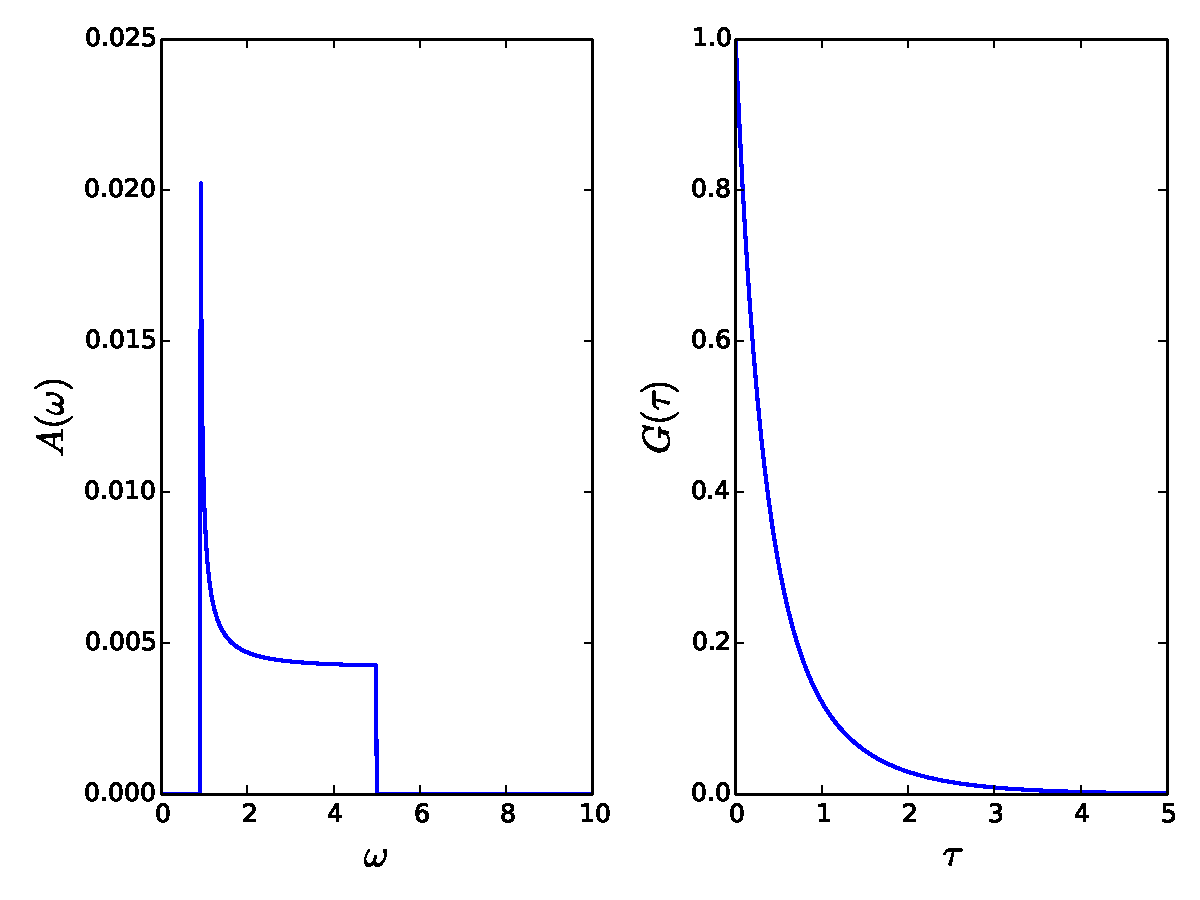
\includegraphics[width=0.95\textwidth]{./images/BCS_A_G_example.pdf}
	\caption{Example BCS spectrum $A(\omega)$ (left) and resulting Greens function $G(\tau)$ (right). The spectrum is calculated according to Equ. \ref{results:equ.1} with $\Delta = 0.9$ and $W = 10$.}
	\label{results:fig.1}
\end{figure}
\FloatBarrier
\subsection*{Influence of $\alpha$}
In the following we investigate the influence of $\alpha$.
We found that the results obtained by MEM highly depend on the regularization parameter $\alpha$. We demonstrate the influence of $\alpha$ by estimating the spectrum shown in Fig. \ref{results:fig.1} for three different values for $\alpha = 0.5,5,50$. The results are shown in Fig. \ref{results:fig.2}
\begin{figure}[htbp]
	\centering
	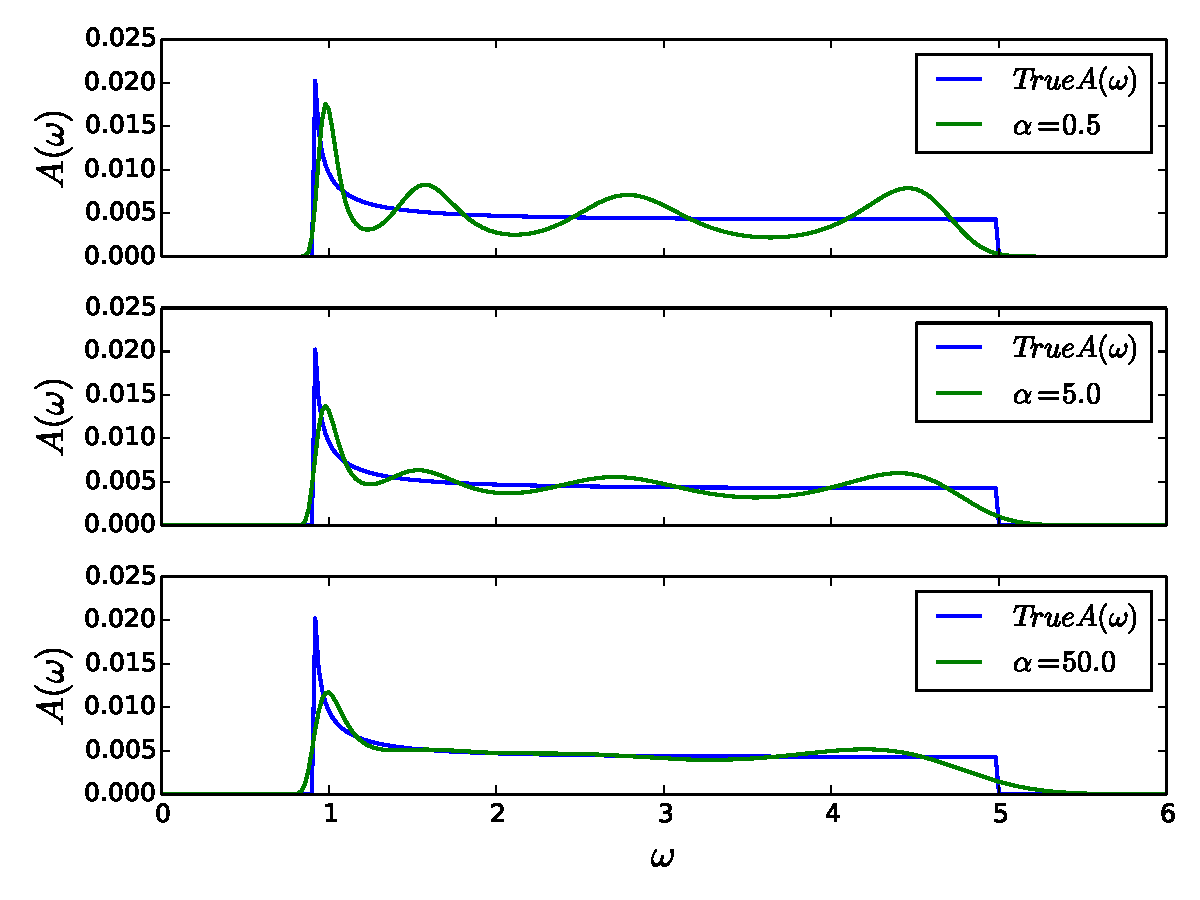
\includegraphics[width=0.95\textwidth]{./images/BCS_varying_alpha.pdf}
	\caption{Influence of the regularization parameter $\alpha$ on the performance of the Maximum Entropy method. The spectrum is calculated according to Equ. \ref{results:equ.1} with $\Delta = 0.9$ and $W = 10$.}
	\label{results:fig.2}
\end{figure}
\FloatBarrier
We observe that for increasing values of $\alpha$ the oscillation like features in the flat region of the spectrum start to vanish and therefor result in a better approximation of the real spectrum in this region. In contrast, the sharp peak at the beginning of the spectrum gets resolved worse for larger values of $\alpha$. This result resembles very nicely the impact of the regularization parameter $\alpha$ on the resulting estimated spectrum. The oscillations due to noise get suppressed at the cost of loosing features like the sharp peak at the beginning of the real spectrum. We further notice that for all three $\alpha$-values the sharp edge at the right end of the spectrum is not resolved very well.
\subsection*{Influence of the singular value threshold $\theta$}
Another important parameter is the choice of the minimum singular value $\theta$ which determines the dimension of the singular space.
Next we investigate the impact of $\theta$ on the performance of the Maximum Entropy method in Fig. \ref{results:fig.3}
\begin{figure}[htbp]
	\centering
	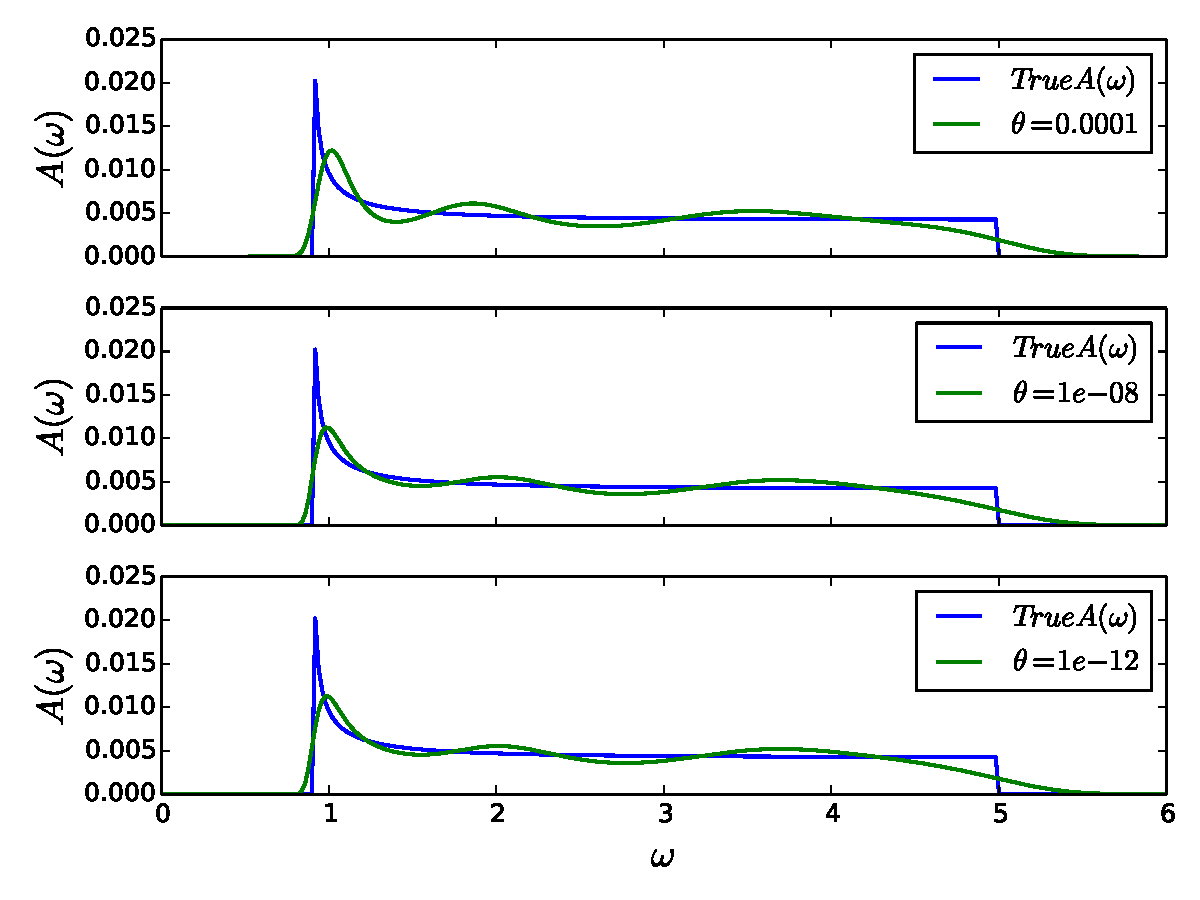
\includegraphics[width=0.95\textwidth]{./images/BCS_varying_cutoffs.pdf}
	\caption{Influence of the minimum singular value $\theta$ on the performance of the Maximum Entropy method. The spectrum is calculated according to Equ. \ref{results:equ.1} with $\Delta = 0.9$ and $W = 10$ and shown in blue in every subplot.}
	\label{results:fig.3}
\end{figure}
\FloatBarrier
Here we see that choosing a very high value for $\theta = 10^{-2}$ results in a wrong approximation of the true spectrum. Whereas reducing $\theta$ to $10^{-3}$ already results in a great improvement on the estimated spectrum. For smaller values of $\theta = 10^{-5},10^{-10},10^{-15}$ there are practically no differences while we can observe that for all of this values the first peak of the BCS spectrum gets resolved better than for $\theta = 10^{-3}$.\

\subsection*{Approaches for $\alpha$}

Now we show the difference between classic MEM and the Bryan method in choosing $\alpha$. As discussed in the theory part the classic MEM uses the maximum value of the probability of $\alpha$ given $A$ and $G$ while Bryan calculates the final $\hat{A}$ by  $\hat{A} = \int A(\alpha) P_{\alpha} d\alpha$. In Fig.~\ref{results:fig.4} we show the probability $p_{\alpha}$ and the resulting spectra calculated by classic and Bryan's method
\begin{figure}[htbp]
	\centering
	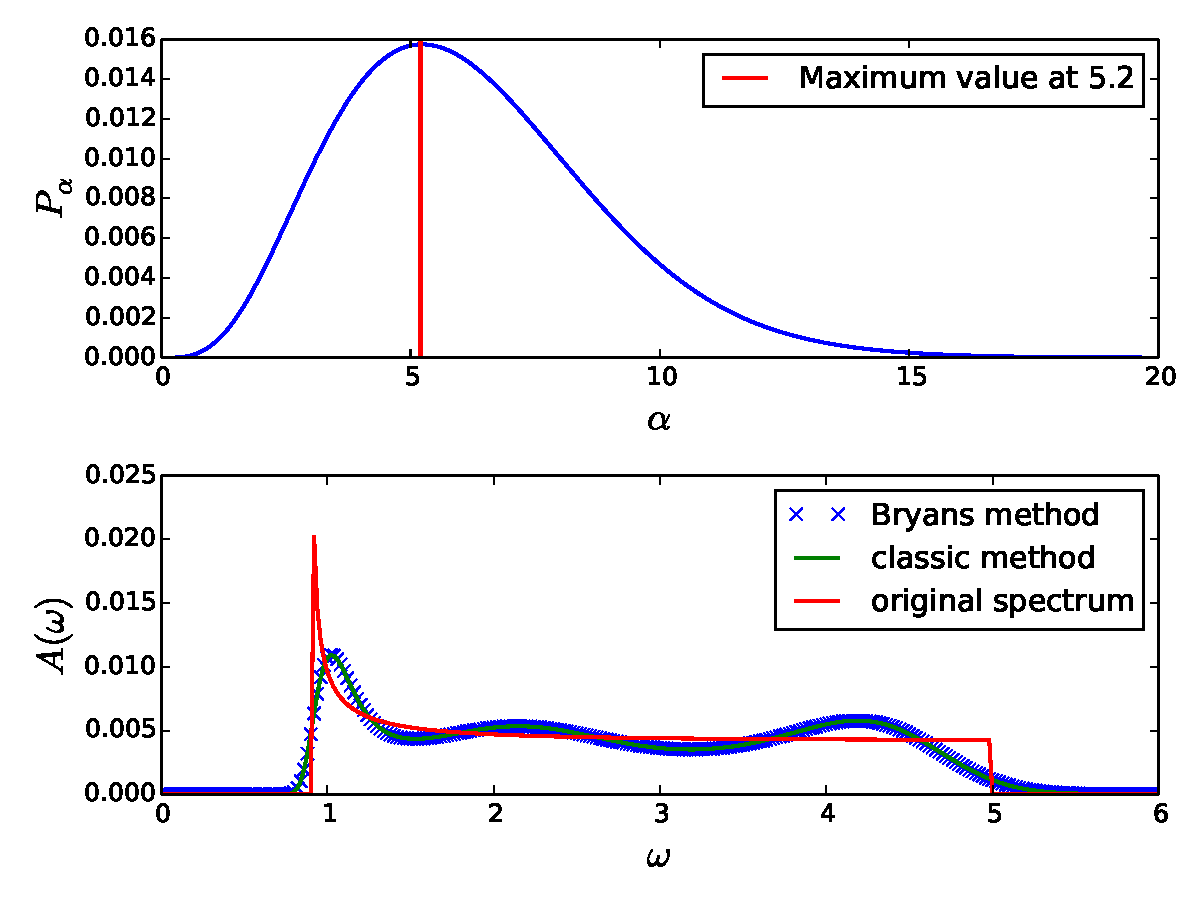
\includegraphics[width=0.95\textwidth]{./images/BCS_Bryan_classic_p_alpha.pdf}
	\caption{Upper row: probability distribution of $\alpha$ for steps of 0.1 in $\alpha$ from 0.5 to 20. lower row: resulting spectra using the classic method and Bryan's method}
	\label{results:fig.4}
\end{figure}
\FloatBarrier
There is practically no visible difference between the classic method and Bryan's method for this data. We suspect this to be at least partly due to the fact, that for $\alpha$ values larger and equal the maximum value of $P_{\alpha}$ the resulting spectra do not change much and only for small values of $\alpha$ we see significant differences in the resulting spectrum. We therefor will perform all following calculations at a constant value of $\alpha = 5$.
We have found empiricaly that this value lies always in the region where a change in $\alpha$ has nearly no influence on the resulting spectrum.
\subsection*{Influence of the noise}
Next we demonstrate the influence of the relative noise in the green's function $G(\tau)$. We estimate the spectra for four different standard deviations of the noise from $10^{-1}$ to $10^{-4}$. To get comparable results we use always the same noise sample  multiplied by the respective relative noise strengths.The results are shown in Fig. \ref{results:fig_5}
\begin{figure}[htbp]
	\centering
	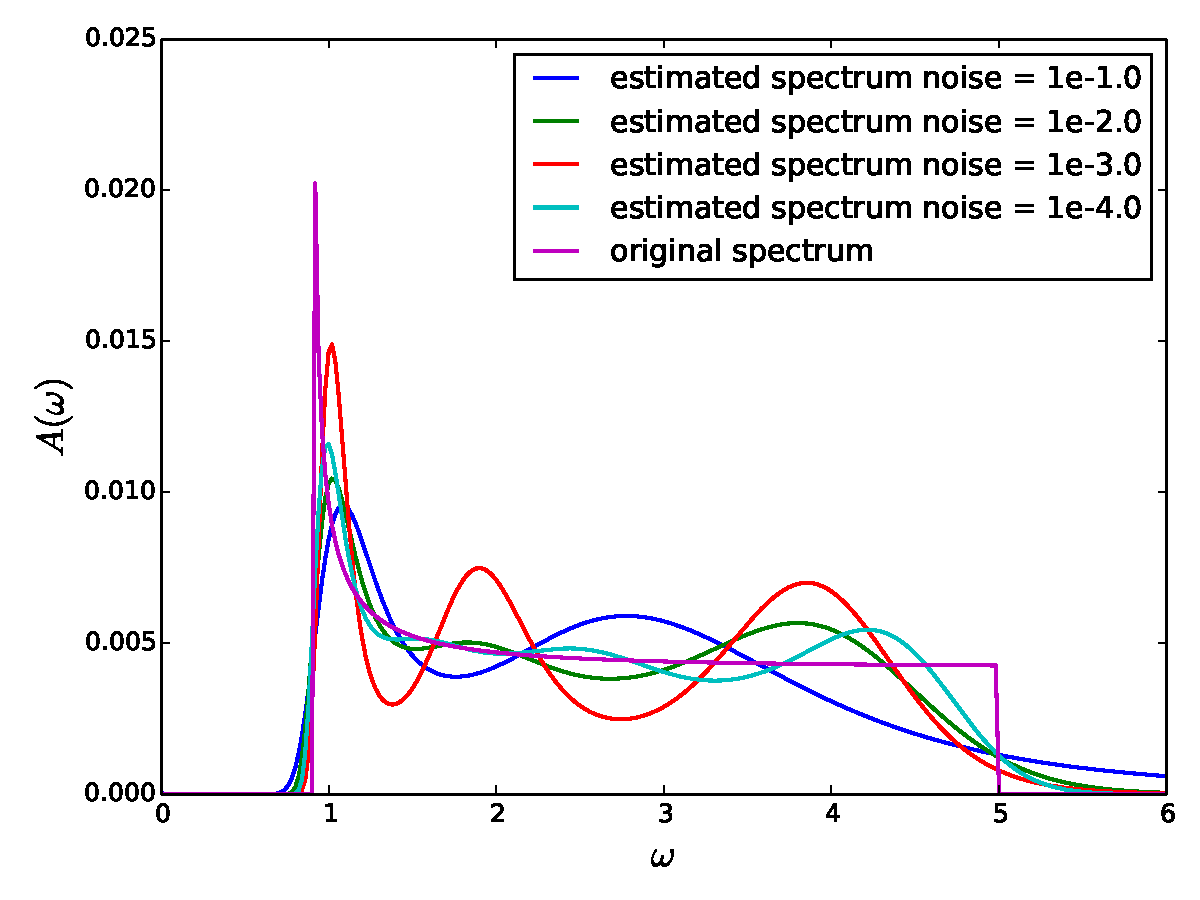
\includegraphics[width=0.95\textwidth]{./images/BCS_varying_noise.pdf}
	\caption{Resulting spectra $A(\omega)$ for four different noise standard deviations.}
	\label{results:fig_5}
\end{figure}
\FloatBarrier
As one would expect in general the estimation of the spectrum becomes better for decreasing noise. For a standard deviation of 10\% of the true greens function data we hardly recover the main features of the true spectrum. For values of 1\%, 0.1\%  and 0.01\% the sharp peak at the beginning and the edge at the right end of the true spectrum becomes more and more captured by the estimated spectrum.

\subsection*{Influence of the default model}
Finally we investigate the impact of the default model $\vec m$ on the performance of the MEM. On the one hand we show the difference for two noninformative, i.e. constant, models which differ only by a constant factor of 10. On the other hand we introduce information about the true spectrum in $\vec m$ to see if we can achieve more accurate results by this. For example if the gap width $\Delta$ of the BCS spectrum is known one could include this information into the default model $\vec m$. We implement this case by adding a delta peak at the frequency value which maximizes true spectrum on top of the noninformative constant $\vec m$. We show the used default models $\vec m$ in Fig. 6 and the results obtained by using them in Fig. \ref{results:fig_7}
\begin{figure}[htbp]
	\centering
	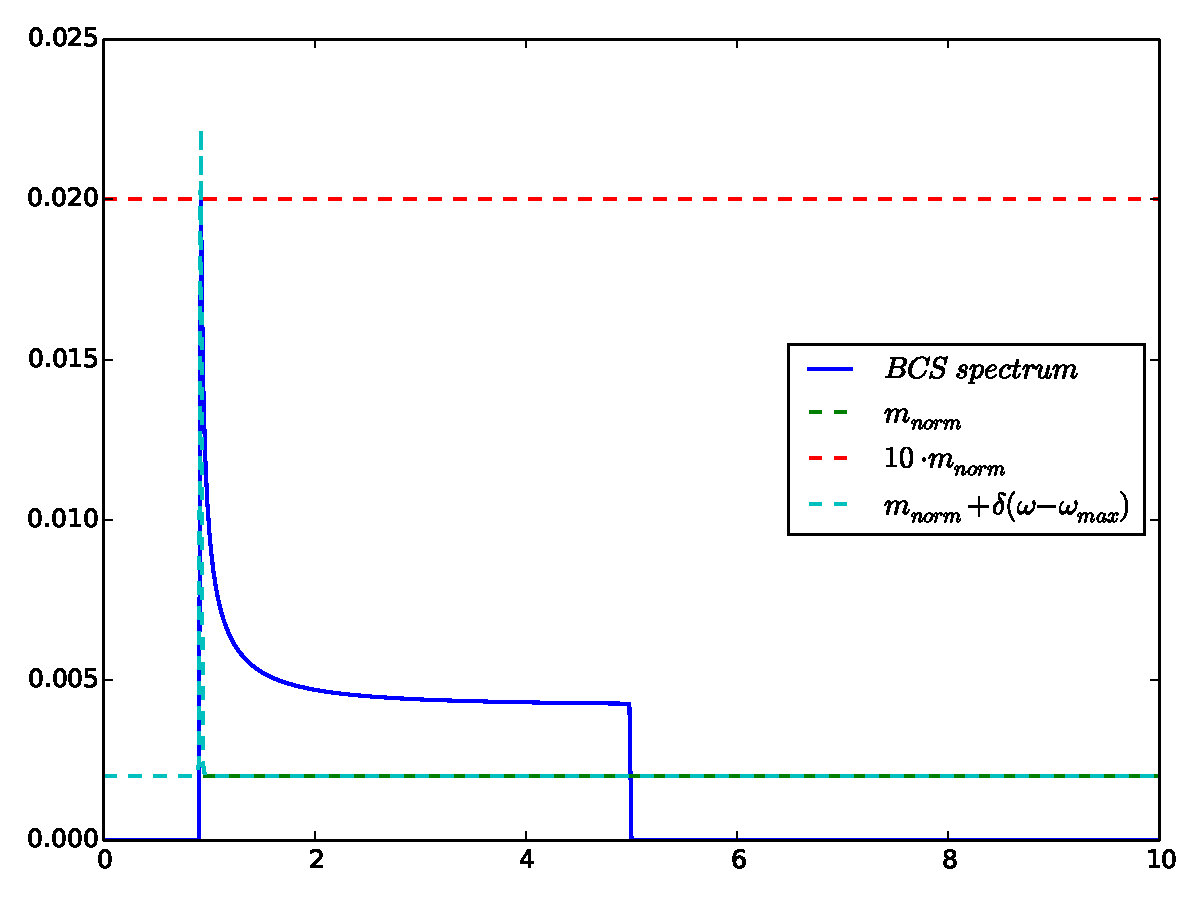
\includegraphics[width=0.95\textwidth]{./images/BCS_different_default_models.pdf}
	\caption{Illustration of the different default models $\vec m$ used.}
	\label{results:fig_6}
\end{figure}
\FloatBarrier
\begin{figure}[htbp]
	\centering
	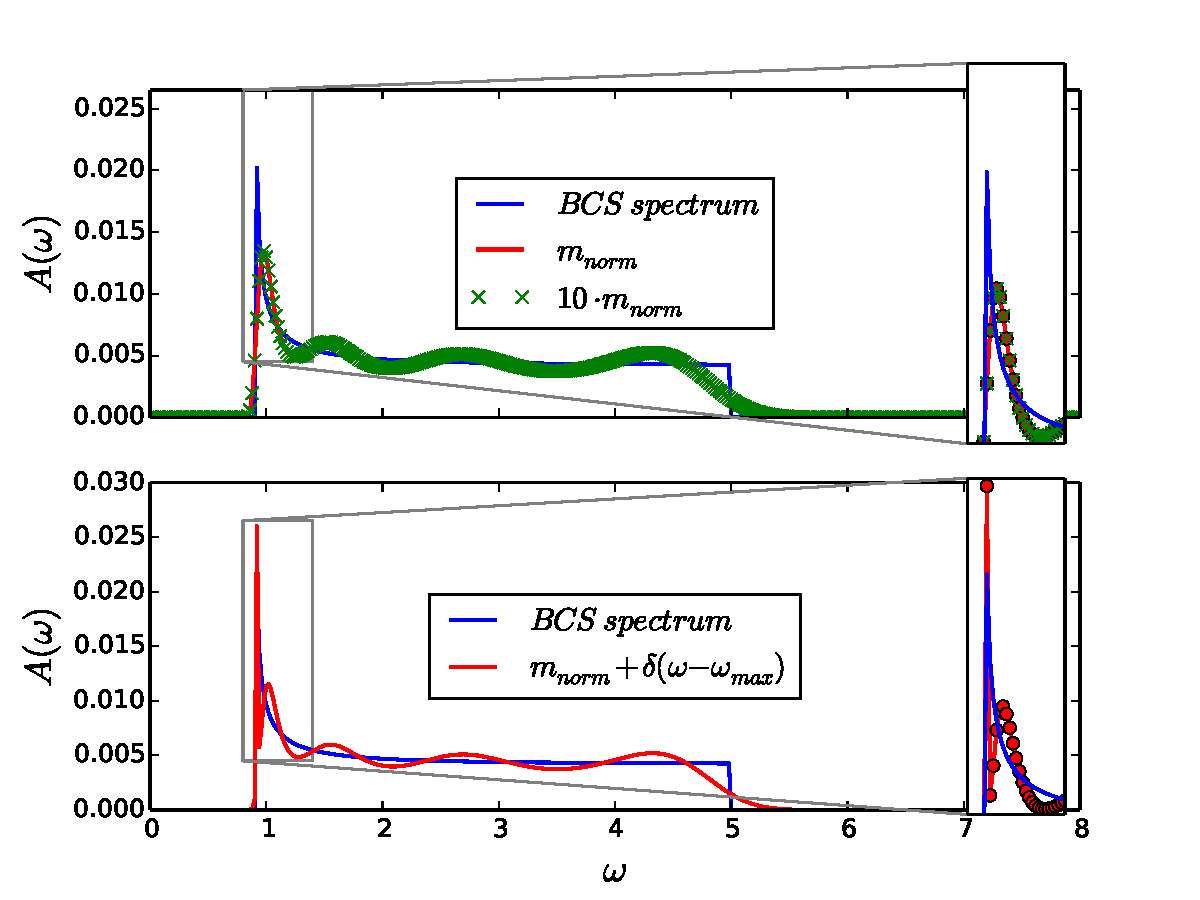
\includegraphics[width=0.95\textwidth]{./images/BCS_delta_peak_example.pdf}
	\caption{Illustration of the effect of $\vec m$ on the performance of the MEM.}
	\label{results:fig_7}
\end{figure}
\FloatBarrier
Surprisingly multiplying $\vec m$ by 10 has no impact on the resulting spectrum (upper plot). This allows us to argue that as long as no information about the true spectrum is known choosing a normalized constant default model is sufficient.
Introducing information in form of a delta peak at the gap width results in a sharp peak at the correct position of the original spectrum. However, one hast to be careful since such strong information as a delta peak will always appear in the estimated spectrum.
